\documentclass[a4paper,12pt]{article}
\usepackage{epsfig,amssymb,amsmath,}
\usepackage{color}

\textwidth=18cm%6.25true in
\textheight=24.5cm%9.65true in
\voffset=-2.5cm%-1true in
\hoffset=-0.75true in

%%%%%%%%%%%%%%%%%%%%%%%%%%%%%%%%%%%%%%%%%%%%%%%%%%%%%%%%%%%%%%%%%%
%\usepackage[sorting=none, url=false, style=numeric-comp]{biblatex}
%\bibliography{../global.bib}
%%%%%%%%%%%%%%%%%%%%%%%%%%%%%%%%%%%%%%%%%%%%%%%%%%%%%%%%%%%%%%%%%%
\usepackage[sort&compress,numbers]{natbib}
\bibliographystyle{apsrev4-1}
\usepackage{doi}%<----------
% https://tex.stackexchange.com/questions/15677
%%%%%%%%%%%%%%%%%%%%%%%%%%%%%%%%%%%%%%%%%%%%%%%%%%%%%%%%%%%%%%%%%%

\usepackage{tikz}
\usetikzlibrary{arrows}
\usepackage[]{hyperref}     
%\hypersetup{citecolor = blue, linktocpage=true}
\usepackage{titlesec}
\titleformat{\subsection}
{\normalfont\large\bfseries}{\thesubsection}{1em}{}

\usepackage{graphicx} % Allows including images    
\graphicspath{{../figures/}, {../figures/growthrates/}}

\usepackage{dcolumn}
\usepackage{array}
\newcolumntype{P}[1]{>{\centering\arraybackslash}p{#1}}
\usepackage{makecell}

\renewcommand{\bf}{\mathbf}
\renewcommand{\cal}{\mathcal}
\newcommand{\pd}[2]{\frac{\partial #1}{\partial #2}}
\newcommand{\pdn}[3]{\frac{\partial^{#3} #1}{\partial #2^{#3}}}
\newcommand{\pdop}[1]{\frac{\partial}{\partial #1}}
\newcommand{\nd}[2]{\frac{d #1}{d #2}}
\newcommand{\ndn}[3]{\frac{d^{#3} #1}{d #2^{#3}}}
\newcommand{\ndop}[1]{\frac{d}{d #1}}
\newcommand{\dt}{\frac{d}{dt}}
\newcommand{\half}{\frac{1}{2}}
\newcommand{\third}{\frac{1}{3}}
\renewcommand{\th}[1]{\frac{1}{#1}}
\newcommand{\ex}[1]{\left\langle #1 \right\rangle}
\renewcommand{\d}{\delta}
\renewcommand{\l}{\ell}
\renewcommand{\t}{\tau}
\newcommand{\ret}{\text{return}}
\newcommand{\tot}{\text{tot}}
\newcommand{\ket}[1]{\left|#1\right\rangle}
\newcommand{\bra}[1]{\left\langle#1\right|}
\newcommand{\braket}[2]{\left\langle#1\middle|#2\right\rangle}
\newcommand{\brakett}[3]{\left\langle#1\middle|#2\middle|#3\right\rangle}
\newcommand{\nn}{\nonumber\\}
\newcommand{\note}[1]{{\color{red}{#1}}}

\DeclareMathOperator{\Tr}{Tr}
\let\Re\relax
\DeclareMathOperator{\Re}{Re}

\title{Thermalization and localization in random unitary circuits}
\author{Charles Stahl}

\begin{document}

\maketitle

\section{Introduction} \label{sec:intro}

In this essay we will discuss the quantum dynamics of closed systems, showing that the two late-time possibilities are thermalization and localization. We will then describe how to study these processes using random unitary circuits. Sec.~\ref{sec:ruc} presents various methods of describing dynamics in thermalizing circuits. The majority of circuits currently described in the literature thermalize, although this is not a necessity. One path to localization in random unitary circuits is through fractonic conservation laws. To motivate these we will introduce fractonic systems in Sec.~\ref{sec:frac} and show how they naturally conserve higher moments of charges. Finally, in Sec.~\ref{sec:fraccirc} we will show that circuits that conserve these higher moments of charge indeed localize. We will follow the results of~\cite{PaiFracton}, and in fact the first 4 sections of this essay are designed to build to these results. Sec~\ref{sec:conc} reviews the broad structure of this essay and presents some possibilities for future research.

\note{Include term ``scrambling, ergodic"}

\note{Always write $S_Z$ as $Z$?}


\section{Quantum dynamics of closed systems} \label{sec:dyn}

This section will serve to introduce the reader to the basics of quantum dynamics of closed systems. It will closely follow Ref.~\cite{Nandkishore14}, drawing on other sources for examples.

I'll cover operator spreading here, although some of that material may belong in the RUC section. Other sources include~\cite{GogolinStatMech, PolkovnikovClosed, Cazalilla2010}.

\subsection{Closed quantum systems} \label{sub:closed}

Quantum statistical mechanics usually considers a quantum system coupled to a bath. As in classical statistical mechanics, this allows the system to exchange energy and conserved charges with the bath. Additionally, the system may become entangled with the bath, leading to dephasing. Then, as in the classical case, the state of the system at long time (is|may be approximated by) the thermal state, $\rho^{\text{th}}(T)=Z^{-1}(T)e^{-H/T}$. 

Sometimes these systems are integrable\dots

\subsection{Thermalization and localization} \label{sub:therm}

Since the bath itself is quantum mechanical, we could consider the system and bath together as a single closed quantum system. We will take this perspective for the remainder of the essay, referring to the original system as some subsystem. The study of closed quantum systems has expanded recently, driven by experimental, numerical, and theoretical motivations~\cite{GogolinStatMech}.

I'll discuss the ETH here as it seems to be an important enough result, but I don't think it's strictly necessary for the flow of the essay.

I'll continue to follow the Nandkishore review for this section and the section on MBL.

\subsection{Operator spreading as a measure of dynamics} \label{sub:opsp}

How can we measure dynamics?
Can we look at how states evolve?
This is tempting, but we would need a background\dots

We will look at how initially local operators spread in time. They will evolve in the Heisenberg picture\dots

Two measures of the spreading of an operator are the right weight density $\rho_R(i,t)$ and the OTOC $C(i,t)$.

\subsection{Other measure of dynamics} \label{sub:other}

Other useful quantity is the bipartite entanglement entropy $S(i,t)$.
Other possible entropies: Renyi entropies.
Dynamics studied in~\cite{RakovskyDiff, HuangRenyi}.
Also mention~\cite{JonayEntanglement}.

I like the transition between thermalizing and localizing phases, so I'll spend some time on that, with sources~\cite{PalHuse, KhemaniCP}. Specifically, the fact that this is not a phase transition of the ground state, like we are used to, and different order parameters for the transition. 

\subsection{Many-body localization} \label{sub:mbl}

If there's time and space\dots


\section{Random unitary circuits and Floquet systems} \label{sec:circuits}

In this essay we will be considering the dynamics of Hamiltonian systems, quantum circuits, and Floquet systems. We have already assumed the reader is familiar with the evolution of operators under Hamiltonian dynamics, but here we will introduce quantum circuits and Floquet systems. Both have unitary evolution, but are in some sense less structured than Hamiltonians.

\note{Define ``physical" systems, disorder realization.}

\note{Haar measure}

\subsection{Random unitary circuits} \label{sub:ruc}

Quantum circuits, unsurprisingly, are the quantum analogue of classical circuits. As unitarity is a constraint on quantum evolution, they are also called unitary circuits. We will be interested in 

\subsection{Floquet systems} \label{sub:floq}

Theres a thorny issue that we brushed asie when we discussed systems without conserved quantities. We defined the systems by their Hamiltonians, but any system with a Hamiltonian conserves energy. As discussed in Sec.~\ref{sec:intro}, random circuits need not have any conserved quantities at all. How then can we compare them to any sort of Hamiltonian system?

The resolution lies in Floquet systems. In this branch of systems, there is a succession of Hamiltonians applied, each for a set amount of time. For example, if we ``turn on" Hamiltonian $H_1$ for time $T/2$ and then $H_2$ for $T/2$, then the Floquet unitary time evolution operator for one whole period of time $T$ is 
\begin{align}
U_F(T) = U_2\left(\frac{T}{2}\right)\; U_1\left(\frac{T}{2}\right) = e^{-i\frac{T}{2}H_2} e^{-i\frac{T}{2}H_1}.
\end{align}
For $t=nT$ with $n\in \mathbb{Z}$, the time evolution operator is $U(t)=U^n(T),$ while for noninteger multiples of $T$ it is more complicated. 

One example is the kicked Ising model~\cite{vonKeyserlingkHydro}, with 
\begin{align}
H_1 &= \phantom{h}\sum_i\left(Z_iZ_{i+1}+gZ_i\right),\nn
H_2 &= h\sum_iX_i. \label{eqn:kicked}
\end{align}
Note that all terms acting at a given time commute with each other. Therefore this Floquet model can be written as a unitary circuit (not random) with 2-site gates. 

Another example, from Refs.~\cite{ZhangFloq, ChenOtoc}, has time evolution operator 
\begin{align}
U_F(T) = e^{-i\frac{T}{2}H_x}e^{-i\frac{T}{2}H_z},
\end{align}
with
\begin{align}
H_x &= \sum_i g\Gamma X_j,\nn
H_z &= \sum_i \left[Z_iZ_{i+1} + (h+g\sqrt{1-\Gamma^2}G_i)Z_i\right],
\end{align}
where $G_i$ are independent Gaussian random variables. We will use the parameters $(g,h,T) = (0.9045,0.8090,0.8)$ throughout.
Note that as $\Gamma\to1$ this approaches the kicked Ising model, which thermalizes. As $\Gamma\to1$, this model becomes equivalent to the time-independent Hamiltonian $H=\sum_i\left[Z_iZ_{i+1} + h_iZ_i\right]$ with random field $h_i$, which is localized. For lack of a better term we will call this the $\Gamma$ model.

As in the previous section, we can study the transition between the localized and thermalizing phases by varying a parameter of the model, in this case $\Gamma$. Fig.~\ref{fig:floqtrans} demonstrates the transition using two diagnostics. 
\begin{figure}
	\centering
	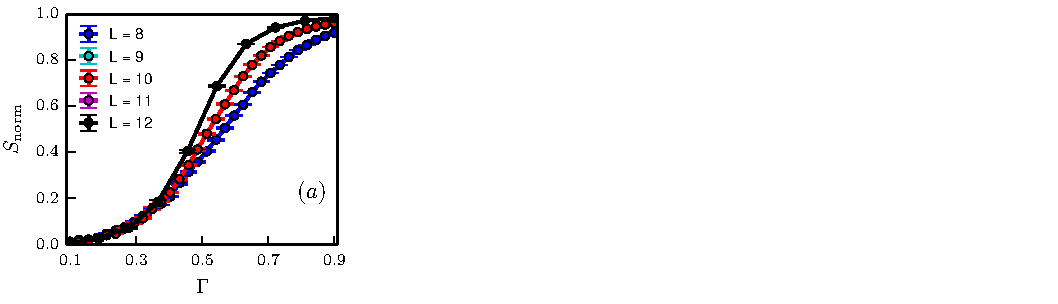
\includegraphics[width=.3\linewidth]{ZhangTransition1}
	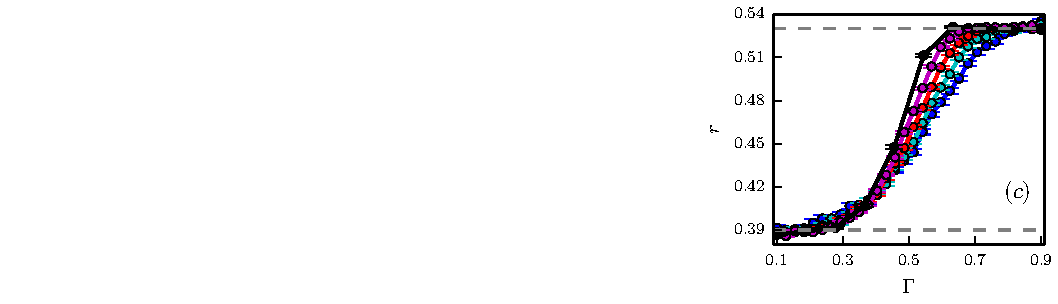
\includegraphics[width=.3\linewidth]{ZhangTransition2}
	\caption{Dynamical phase transition of the $\Gamma$ model. (a) demonstrates the phase transition through the average entanglement entropy between halves of the chain. (c) shows the same transition, but using the level statistics parameter. Figure from~\cite{ZhangFloq}.}
	\label{fig:floqtrans}
\end{figure}
The first is the entanglement entropy between two halves of the chain in energy eigenstates, 
\begin{align}
S_E \equiv -\Tr\{\rho_L\log\rho_L\} = -\Tr\{\rho_R\log\rho_R\},\label{eqn:Shalf}
\end{align}
where $\rho_L$ and $\rho_R$ are reduced density matrices of the right and left halves of the chain, with no relation to the operator right- and left-weights. The second equality in~\ref{eqn:Shalf} is due to the whole chain being in a pure state. The maximal possible entanglement between these halves is $S_\text{max}=L/2$, but random pure states will be close to the Page value~\cite{Page, ZhangTherm}
\begin{align}
S_R = \frac{L}{2} - \th{2\ln 2} -\mathcal{O}\left(\th{2^L}\right).
\end{align}

In the thermalizing phase the eigenstates have ``volume law" entanglement, close to $S_R$, while in the localized phase they have ``boundary law" entanglement, constant in $L$~\cite{ZhangFloq}. Therefore for large enough $L$, $S_E/S_R$ should distinguish between the phases. After averaging over all eigenstates for a given disorder realization and then averaging over disorder realizations, we arrive at $S_\text{norm} = \ex{S_E}/S_R$.

Alternatively we can use the level statistics parameter $r$ discussed previously. In the thermalizing phase the energies should be distributed according to the circular orthogonal ensemble with $r \approx 0.53$, while in the localizing phase the energies follow Poisson level statistics with $r\approx 0.39$. The dashed lines in Fig.~\ref{fig:floqtrans} show these values.

In Fig.~\ref{fig:floqtrans}, notice the agreement between the two diagnostics in the critical value $\Gamma_c$. Furthermore, both transitions become sharper for increasing $L$, as one would expect. The suggestion is that the transition is singular in the thermodynamic limit. In Sec.~\ref{sub:fncons} we will study this model at $\Gamma=.85$, deep in the thermalizing phase.


\section{Thermalization in systems with no conservation laws} \label{sec:ncons}

In this section I'll bring back the concepts of thermalization and show how they can be quantified in random circuits. For the actual construction of circuits I'll use~\cite{NahumRuhmanHuse, NahumEntanglement}.
For operator hydrodynamics I'll cite~\cite{NahumOpSp, vonKeyserlingkHydro, KhemaniLambda, KhemaniOpSp, JonayEntanglement}. Some of this material is not in RUCs though, so I still have to sort that out.

\subsection{Physical systems with no conservation laws} \label{sub:fncons}

As shown previously, the $\Gamma$ model with $\Gamma=0.85$ is deep within the thermalizing phase. Ref.~\cite{ChenOtoc} studied the OTOC of an initially local operator in this model. It uses a \note{slightly different definition of the OTOC...}

The key point is the exponential dependence of the OTO correlator. 
\begin{figure}
	\centering
	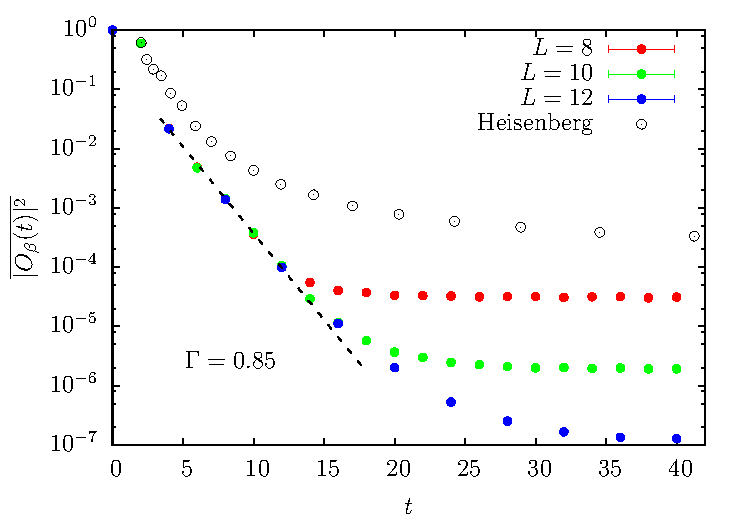
\includegraphics[width=.5\textwidth]{ChenExp}
	\caption{Exponential decay of the OTO correlator in a thermalizing Floquet model with no conserved charges~\cite{ChenOtoc}. For increasing system size, the decay continues to be exponential for a longer time before saturating. The black circles show the non-expenential decay of a Hamiltonian system. This decay is power-law, and will be discussed in the following section.}
	\label{fig:ChenExp}
\end{figure}
Fig.~\ref{fig:ChenExp} shows the exponential decay of the OTO correlator for various system sizes. Finite size effects cause the OTO correlator to saturate and therefore deviate from exponential behavior. However, the figure shows that this happens later for larger $L$, suggesting that the exponential decay continues for an arbitrarily long time for large enough $L$.

Ref.~\cite{vonKeyserlingkHydro} cranks $\Gamma$ all the way to 1, to study the kicked Ising model, defined in Eq.~\ref{eqn:kicked}. It goes beyond the early-time exponential dependence to study the saturation. The quantity under inspection is now the OTOC rather than the OTO correlator, so it should start at 0 and saturate to 1. There is also a focus on the operator right- and left-weights, $\rho_L$ and $\rho_R$.

Fig.~\ref{fig:vonKSpreading} shows the relevant quantities. Although it is for the quantum circuit, the qualitative behavior is the same (that's the whole point of this essay). At each site, exponential growth of both $\rho_R$ and the OTOC begins when the site enters the light cone. Exponential growth continues until the front reaches the site, at which point $\rho_R$ peaks and the OTOC begins to saturate. This front is the focus of Ref.~\cite{vonKeyserlingkHydro}.
Figs.~\ref{fig:vonKSpreading}~(a) and (b) can be thought of as horizontal slices though Fig.~\ref{fig:vonKSpreading}~(c). To compare with Fig.~\ref{fig:ChenExp}, imagine a vertical slice through~\ref{fig:vonKSpreading}~(c), with $t=0$ occurring at the position of the light cone.

The results, found through numerical simulation, are that the front propogates linearly at a velocity called the butterfly velocity, $v_B$. Consider $\rho(i,t)$. For $t<<v_B i$, the spreading operator has not yet reached $i$ and $\rho(i,t)$ is small. As the peak passes site $i$, a significant number of Pauli strings in the operator end on $i$. In the future, most strings end after $i$ so $\rho_R(i)$ is again small. For a given $t$, $\rho_R(i)$ peaks at $i=v_B t$. This peak has width $\sim t^\alpha$~\cite{vonKeyserlingkHydro}.
\begin{figure}
	\centering
	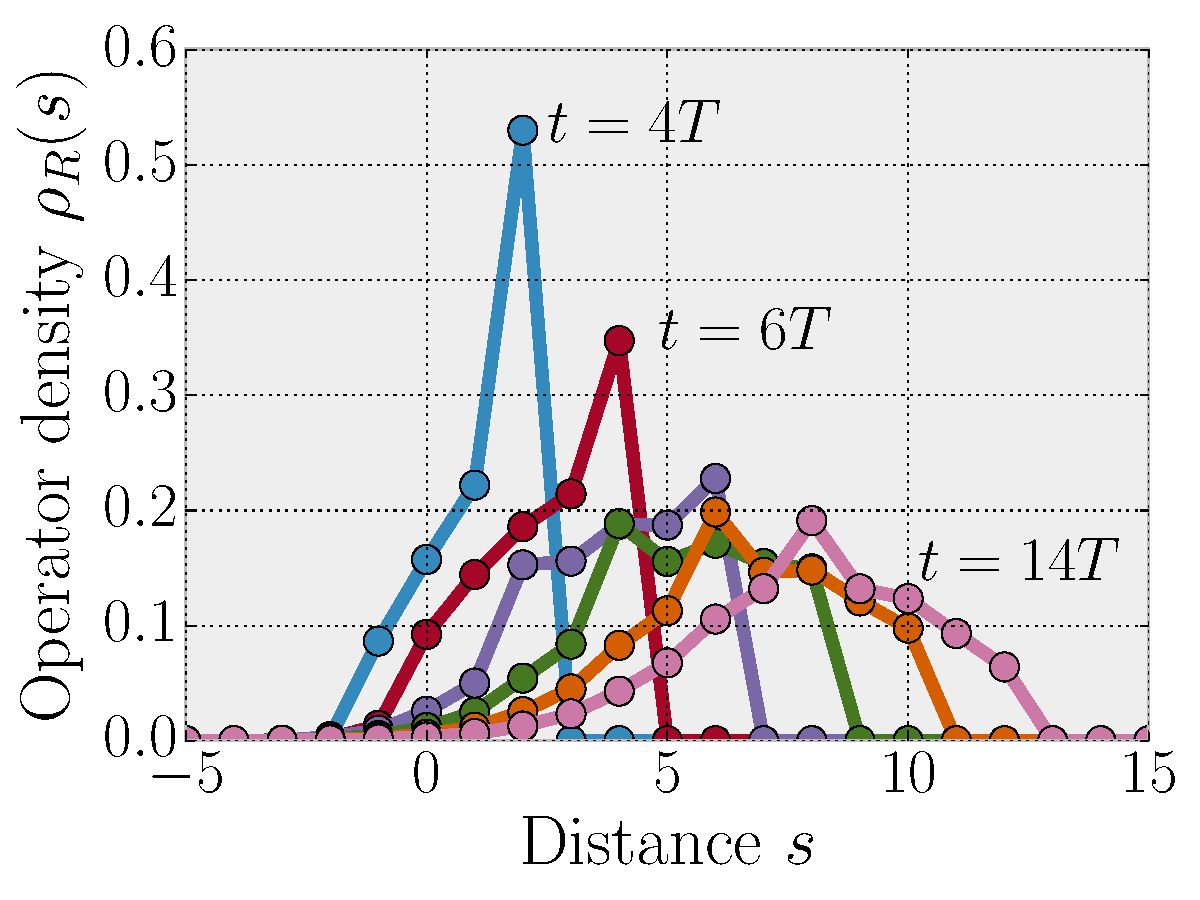
\includegraphics[width=.3\textwidth]{vonKpeaks}
	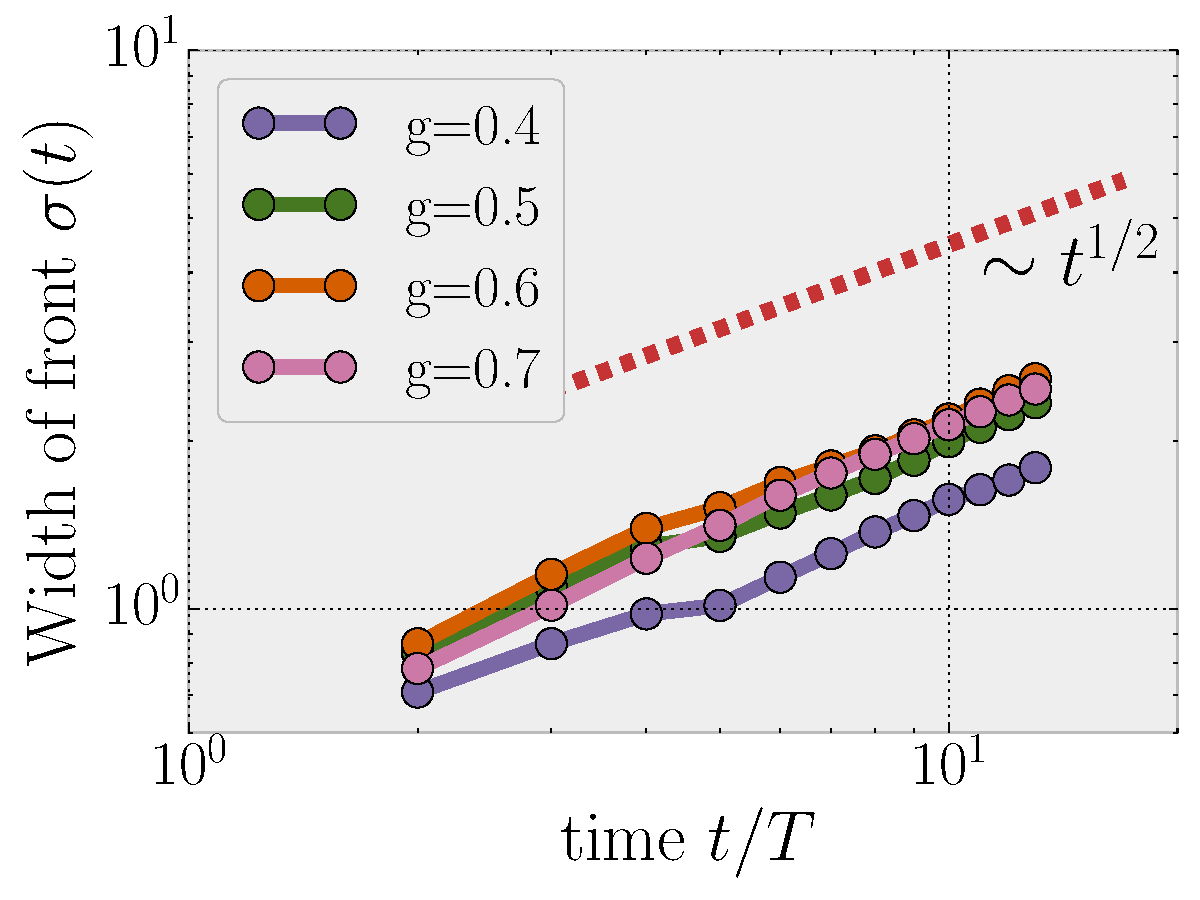
\includegraphics[width=.3\textwidth]{vonKalpha}
	\caption{Spreading of peaks in the kicked Ising model~\cite{vonKeyserlingkHydro}.}
	\label{fig:vonKalpha}
\end{figure}
Fig.~\ref{fig:vonKalpha} shows that $\alpha\approx .5$, so that the peaks spread with $\sqrt{t}$. This will be another test of our quantum circuits.

\subsection{Circuits with no conservation laws} \label{sub:cncons}

Early exponential growth.
Presence of front.
Broadening of front and exponential dependence therein.

The circuit under investigation in this section has the same architecture as Fig.~\ref{fig:circuit}, with each gate chosen from the Haar measure. Our goal is to find the dynamics of $\rho_R$ under the action of the full circuit, and our analysis will follow~\cite{vonKeyserlingkHydro}. The first step in doing so is to calculate the dynamics of $\rho_R$ under a single gate. 

We want to calculate $\rho_R(i,\tau+1)$ and $\rho_R(i+1, \tau+1)$ (Fig.~\ref{fig:2sites}). It should be clear that these quantities only depend on $\rho_R(i,\tau)$ and $\rho_R(i+1, \tau)$. In fact it is even simpler, in that $\rho_R(i,\tau+1)$ and $\rho_R(i+1, \tau+1)$ only depend on the sum $\rho_R(i,\tau) + \rho_R(i+1, \tau)$. 

\begin{figure}
	\centering
	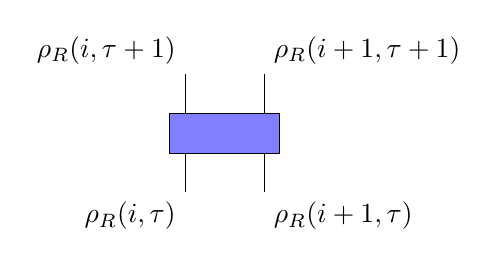
\begin{tikzpicture}[scale = 1]
\draw (0,0) node[below left]{$\rho_R(i,\tau)$} -- (0,1.5) 
			node[above left]{$\rho_R(i,\tau+1)$};
\draw (1,0) node[below right]{$\rho_R(i+1,\tau)$} -- (1,1.5)
			node[above right]{$\rho_R(i+1,\tau+1)$};

\filldraw[color=black, fill=blue!50] (-.2,.5) rectangle (1.2,1);


\end{tikzpicture}
	\caption{Diagram of the operator weights before and after the application of the gate. Values at $\t+1$ are calculated in the text.}
	\label{fig:2sites}
\end{figure}

Looking at $\rho_R(i,\tau)$ and $\rho_R(i+1, \tau)$ is equivalent to looking only at Pauli strings which are $I$ on all sites past $i+1$ but are non-identity on either $i$ or $i+1$ (or both).
This leaves us with $q^4-1$ two-site operators to consider. The Haar-random gate transforms any of these operators to any other with equal probability~\cite{BrownScrambling}, regardless of whether the initial operator was an identity on site $i+1$. This is why the final values only depend on $\rho_R(i,\tau) + \rho_R(i+1, \tau)$.

Of the $q^4+1$ final operators, $q^2-1$ are the identity on site $i+1$. These operators contribute to $\rho_R(i,\tau+1)$, while the rest contribute to $\rho_R(i+1, \tau+1)$. In other words the weight moves to site $i$ with probability $p_\text{back} = \frac{q^2-1}{q^4-1} = \th{q^2+1}$ or moves forward with probability $p\equiv 1- p_\text{back} = \frac{q^2}{q^2+1}$. Thus
\begin{align}
\rho(i,\t+1) &= (1-p)\left[\rho(i,\t)+\rho(i+1,\t)\right],\nn
\rho(i+1,\t+1) &= p\left[\rho(i,\t)+\rho(i+1,\t)\right].
\end{align}
This is true at each individual gate. If there were a gate at each site at each time, this would be the final word. However, since the dynamics will only be periodic in every two layers of the circuit, we must calculate the dynamics for two layers to get the whole picture.

To do so, we will define some dense but useful notation. Since the sum of weights at consecutive sites is so important, we will abbreviate it as
\begin{align}
\tilde{\rho}_R(i,\t) \equiv \rho_R(i,\tau) + \rho_R(i+1, \tau). \label{eqn:rhotil}
\end{align}
We will want to find $\tilde{\rho}_R(i,\t+2)$. To do so we find
\begin{align}
\rho_R(i-1, \t+1) &=    p  \tilde{\rho}_R(i-2, \t),\nn
\rho_R(i  , \t+1) &= (1-p) \tilde{\rho}_R(i  , \t),\nn
\rho_R(i+1, \t+1) &=    p  \tilde{\rho}_R(i  , \t),\nn
\rho_R(i+2, \t+1) &= (1-p) \tilde{\rho}_R(i+2, \t).\label{eqn:4sites1}
\end{align}
Similar calculation at time $\t+2$ result in
\begin{align}
\rho_R(i  , \t+2) &= p^2\tilde{\rho}_R(1-2,\t) + p(1-p)\tilde{\rho}_R(i,\t),\nn
\rho_R(i+1, \t+2) &= p(1-p)\tilde{\rho}_R(i,\t) + (1-p)^2\tilde{\rho}_R(i+2,
	\t), \nn
\tilde{\rho}_R(i,\t+1)&=p^2\tilde{\rho}_R(i-2,\t)+2p(1-p)\tilde{\rho}_R(i,\t)+
	(1-p)^2\tilde{\rho}_R(i+2,\t). \label{eqn:4sites2}
\end{align}
Fig.~\ref{fig:4sites} shows a diagram containing these values.
\begin{figure}
	\centering
	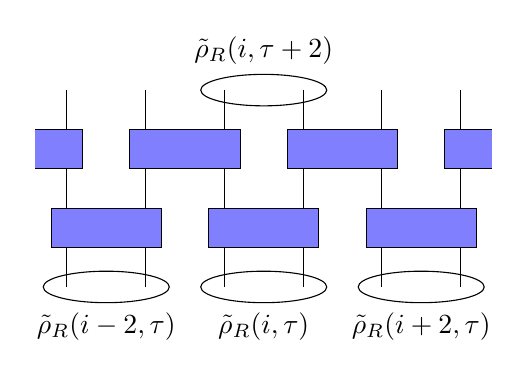
\begin{tikzpicture}[scale = 1]
\draw (0,0) -- (0,2.5);
\draw (1,0) -- (1,2.5);
\draw (2,0) -- (2,2.5);
\draw (3,0) -- (3,2.5);
\draw (4,0) -- (4,2.5);
\draw (5,0) -- (5,2.5);

\foreach \x/\y in {0/1, 2/1, 4/1, 1/2, 3/2} 
\filldraw[color=black, fill=blue!50] (\x-.2,\y-.5) rectangle (\x+1.2,\y);

\draw (0.5,0) circle [x radius=.8, y radius=.2];
\draw (0.5,-0.2) node[below]{$\tilde{\rho}_R(i-2,\t)$};
\draw (2.5,0) circle [x radius=.8, y radius=.2];
\draw (2.5,-0.2) node[below]{$\tilde{\rho}_R(i,\t)$};
\draw (2.5,2.5) circle [x radius=.8, y radius=.2];
\draw (2.5,2.7) node[above]{$\tilde{\rho}_R(i,\t+2)$};
\draw (4.5,0) circle [x radius=.8, y radius=.2];
\draw (4.5,-0.2) node[below]{$\tilde{\rho}_R(i+2,\t)$};

\draw[fill=blue!50] (-.4,1.5) -- (.2,1.5) -- (.2,2) -- (-.4,2);
\draw[fill=blue!50] (5.4,2) -- (4.8,2) -- (4.8,1.5) -- (5.4,1.5);

\end{tikzpicture}
	\caption{Operator weights after two layers of the circuit}
	\label{fig:4sites}
\end{figure}

The fact that $i\pm1$ and $\t\pm1$ do not appear in Eq.~\ref{eqn:4sites2} demonstrates the usefulness of the coarse-grained variables, defined in Fig.~\ref{fig:circuit}. Switching to those variable and dropping the tilde, Eq~\ref{eqn:4sites2} becomes
\begin{align}
\rho_R(x,t+1)&=p^2\rho_R(x-1,t)+2p(1-p)\rho_R(x,t)+(1-p)^2\rho_R(x+1,t), 
	\label{eqn:4sites3}
\end{align}
which is the equation for a biased random walk that steps to the right with probability $p^2$ and to the left with probability $(1-p)^2$, otherwise staying at the same site. 

Therefore, for any operator initially local at position $x_0$, $\rho_R$ spreads linearly with a front located near position $x = x_0 + v_B t$. The front spreads diffusively as $\ex{x^2}-\ex{x}^2=2Dt$~\cite{vonKeyserlingkHydro}. The values are
\begin{align}
v_B &= p^2-(1-p)^2 = \frac{q^2-1}{q^2+1},\nn
D   &= \sqrt{1-v_B^2}/4 = \frac{q/2}{q^2+1}.
\end{align}
These results can be summarized in Fig.~\ref{fig:vonKSpreading}.
\begin{figure}
	\centering
	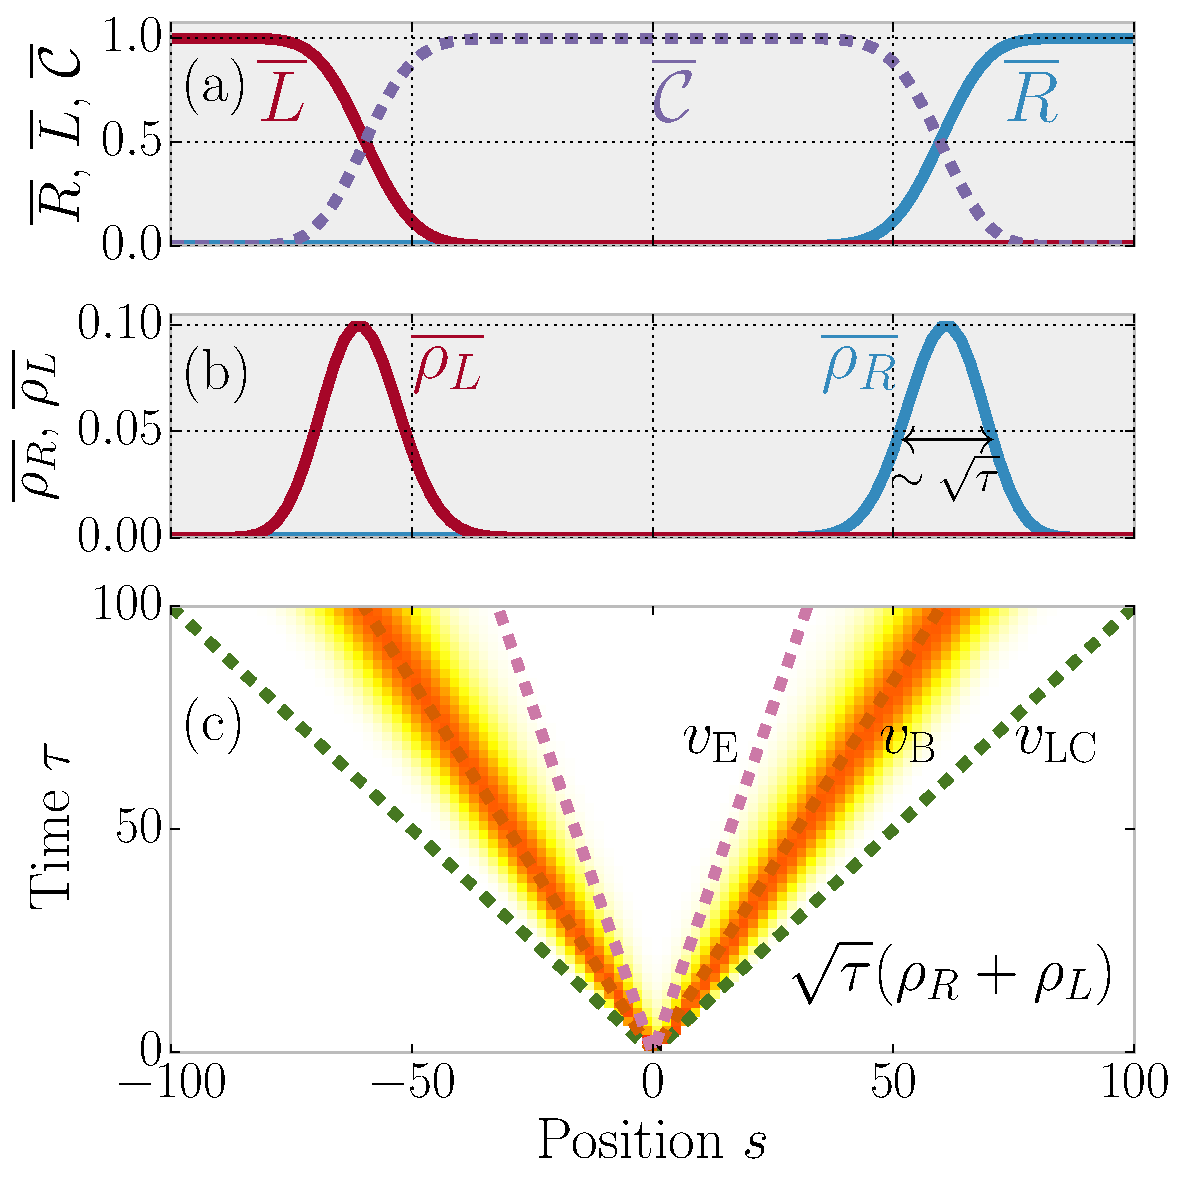
\includegraphics[width=.5\textwidth]{vonKSpreading}
	\caption{Spreading of an initially local operator under a quantum circuit with no conservation laws~\cite{vonKeyserlingkHydro}.}
	\label{fig:vonKSpreading}
\end{figure}
As an interesting aside, note that in the large $q$ limit the front does not diffuse and $v_B=1$, the lightcone velocity~\cite{NahumOpSp}.

The important features that we can match to the behavior of the floquet model are the exponential growth at early time and the behavior of the front of the spreading operator. As in the kicked Ising model, we have shown that the front moves linearly. The diffusion process has a width $\sim \sqrt{Dt}$, which is to say $\alpha=0.5$

\note{vonKeyserlingk page 6.}


\section{Thermalization in systems with conservation laws} \label{sec:cons}

Introducing conserved charges to our systems slows down their dynamics. In this section we will see how this process occurs, in both physical systems and quantum circuits. It is straightforward to introduce conserved charges to the circuits by restricting to gates that satisfy some conservation law. For the physical systems we have two ways to proceed. We can either consider Floquet systems with conservation laws, or systems with time-independent Hamiltonians (with or without further conservation laws).

\subsection{Floquet systems with conserved quntities} \label{sub:fcons}

We can introduce conserved charges to Floquet systems by ensuring that both partial Hamiltonians in the model obey some conservation law. Ref.~\cite{KhemaniOpSp} studies a model with time evolution operator
\begin{align}
U_F(T)=e^{i\frac{T}{2}H_z}e^{i\frac{T}{2}H_{xy}},
\end{align}
where
\begin{align}
H_z &= J_z\sum_i Z_iZ_{i+1},\nn
H_{xy} &= J_{xy}\sum_i\left[X_iX_{i+1}+Y_iY_{i+1}\right].
\end{align}

\note{In these ``physical systems," it is possible to have approximately conserved charges, i.e. on the localized side of a phase transition\dots}

\subsection{Circuits with conservation laws} \label{sub:ccons}

\note{ballistic front,
	a power-law tail behind the front, and diffusively spread-
	ing charges near the origin}


\section{Fractonic systems} \label{sec:frac}

In this section we will explore various fractonic systems. We will start with exactly solvable models and show that these naturally result in massive (gapped) fractons. However we will quickly transition to tensor gauge theory, where we can create gapless fractons. Ultimately, we want to show the connection between multipole conservation laws (specifically dipole) and fractons. This motivates the study of random circuits that conserve dipole moment as a setting for localized charges, which will be presented in Sec.~\ref{sec:fraccirc}.

The conservation of dipole moment means that an isolated charge cannot move without creating an isolated dipole somewhere else, which costs energy. Thus, the charges are immobile in the low-energy limit. 

\subsection{Tensor gauge theory} \label{sub:tensor}

We will show how fracton conservation laws naturally lead to tensor gauge theory. Although this is not strictly necessary to understand the dynamics of fracton systems, the literature often refers to fractons using the language of tensor gauge theory. This discussion follows the treatment in~\cite{PretkoFractonGauge}. 

To start, we will briefly review the familiar form of U(1) gauge theory. Consider a complex scalar field $\phi(x,t)$. We will treat time and space separately despite the theory being Lorentz invariant because the fracton theory is not Lorentz invariant. The charge density of this field is $\rho =\phi^\dag\phi$, with total charge $Q=\int d^dx \rho$. Requiring $Q=\text{const.}$ is equivalent to \note{requiring
\begin{align}
\phi\to e^{i\alpha}\phi
\end{align}	
be a symmetry of the theory,} for constant $\alpha$. At this point $\phi$ and all of its derivatives and powers transform covariantly, which is to say that each operator transforms as $\mathcal{O}\to e^{in\alpha}\mathcal{O}$ under the phase rotation.

Gauging this theory requires that the theory be invariant under $\phi\to e^{i\alpha(x,t)}\phi$ for arbitrary $\alpha(x,t)$. However, the derivative of the field now transforms as 
\begin{align}
\partial_i\phi\to e^{i\alpha}\left(\partial_i+\partial_i\alpha\right)\phi,\nn
\partial_t\phi\to e^{i\alpha}\left(\partial_t+\partial_t\alpha\right)\phi.
	\label{eqn:nconv}
\end{align}
This is not a covariant transformation, as it mixes the derivatives of $\phi$ with $\phi$ itself. The standard solution is to introduce gauge derivatives $D_i=\partial_i-iA_i$ and $D_t=\partial_t-i\Phi$, where $\Phi$ recalls the notation for the scalar potential of electromagnetism. We then have 
\begin{align}
D_i\phi\to e^{i\alpha}D_i\phi,\nn
D_t\phi\to e^{i\alpha}D_t\phi,
\end{align}
if 
\begin{align}
A_i &\to A_i+\partial_i\alpha, \nn
\Phi&\to\Phi+\partial_t\alpha.
\end{align}
We can then go on to calculate field strengths and possible terms in the action, but our main interest is in the fact that the gauge field is a spacetime vector $A_\mu=(\Phi,A_i)$. For more details see~\cite{PretkoFractonGauge}.

We will now go through the same steps for a fracton field $\phi$ in order to show the natural emergence of symmetric tensor gauge fields. $\phi$ is again a complex scalar that conserves charge $Q=\int d^dx\rho$. It also conserves dipole moment $P_i = \int d^dx\rho x^i$ (breaking Lorentz invariance). Together these correspond to phase rotations of the form 
\begin{align}
\phi\to e^{i\alpha+i\lambda_ix^i}\phi.
\end{align}
We will write this phase as $e^{i\alpha(x)}$ where $\alpha$ is restricted to be linear until we gauge the theory.

Now $\partial_i\phi\to e^{i\alpha}(\partial_i+\lambda_i)\phi$ is no longer covariant. The second derivative 
\begin{align}
\partial_i\partial_j\phi\to e^{i\alpha}(\partial_i\partial_j+\lambda_i\partial_j+\lambda_j\partial_i)\phi
\end{align}
looks slightly more promising because its symmetric structure can also be obtained from the operator $\partial_i\phi\partial_j\phi$. In fact, the lowest order operator is~\cite{PretkoFractonGauge}
\begin{align}
\phi\partial_i\partial_j\phi-\partial_i\phi\partial_j\phi \to e^{2i\alpha} \left(\phi\partial_i\partial_j\phi-\partial_i\phi\partial_j\phi\right).
\end{align}
This means that the action can contain this operator.

Gauging the fracton theory so that $\alpha$ is again an arbitrary function, we now find
\begin{align}
\phi\partial_i\partial_j\phi-\partial_i\phi\partial_j\phi \to e^{2i\alpha} \left(\phi\partial_i\partial_j\phi-\partial_i\phi\partial_j\phi + i(\partial_i\partial_j\alpha)\phi^2\right).
\end{align}
This suggests that, instead of constructing the covariant first derivative $D_i\phi$, we construct a covariant second derivative 
\begin{align}
D_{ij}\phi^2=\phi\partial_i\partial_j\phi-\partial_i\phi\partial_j\phi + iA_{ij}\phi^2,
\end{align}
where this is shorthand for $D_{ij}$ being a bilinear derivative operator acting on two copies of the field $\phi$. This operator transforms covariantly if 
\begin{align}
A_{ij}\to A_{ij}+\partial_i\partial_j\alpha.
\end{align}
This transformation law requires $A_{ij}$ to be symmetric, and we have found our symmetric tensor gauge field. 

The theory still contains a scalar gauge field $\Phi\to\Phi+\partial_t\alpha$. For the construction of the lowest order Lagrangian of this theory, and other possible symmetric tensor gauge theories, see~\cite{PretkoFractonGauge}.

\subsection{More on fractons} \label{sub:morefrac}

(I'll then discuss this model more, including the difference between the discrete and continuous cases. I'll also present some of the connections to elasticity and gravity, such as in~\cite{PretkoElasticity}.)


\section{Localization in fractonic circuits} \label{sec:fraccirc}

This section will mostly cover the results in~\cite{PaiFracton}. I'll go through their analytic results and show that their numerics match up. I'd prefer not to do my own numerics because I assume anything I can do in the next month and a half will be a subset of what they achieved, but if you think my essay would benefit from some validation of their numerics at lower $L$, then I'll go for it. 

Since the dipole density is a conserved charge whose higher moments are not conserved, it should behave the way that charge density did in the ergodic charge conserving circuit.

The entirety of this section is based on the work in~\cite{PaiFracton}.

\subsection{Random walks in $d=1$} \label{sub:walks}

The diffusion operator is $\mathcal{D} = \partial_t-D\partial_x^2$, where $D$ is the diffusion constant. Consider the function $G(x,t)=(4\pi Dt)^{-d/2} e^{-x^2/4Dt}$. We can see that $\mathcal{D}G(x,t)=0$ for $t>0$ 
\begin{align}
\partial_t G(x,t) &= \phantom{D}(4\pi D)^{-\frac{d}{2}} \left[-\frac{d}{2} 
	t^{-\frac{d}{2}-1} + t^{-\frac{d}{2}}\frac{x^2}{4Dt^2} \right]
	e^{\frac{-x^2}{4Dt}},\\
D\partial_x^2 G(x,t) &= D(4\pi D)^{-\frac{d}{2}} \vec{\partial_x}\cdot 
	\frac{-\vec{x}}{2Dt}e^{\frac{-x^2}{4Dt}} \nn
&= D(4\pi D)^{-\frac{d}{2}} \left[-\frac{d}{2D} 
	t^{-\frac{d}{2}
	-1} + t^{-\frac{d}{2}}\frac{x^2}{4D^2t^2} \right]e^{\frac{-x^2}{4Dt}}, \\ 
\mathcal{D}G(x,t) &= 0.
\end{align}
Furthermore, at early time we have $G(x,t)\xrightarrow[t\to0]{}\delta(x)$:
\begin{align}
G(x,0) = 0, \quad x\ne 0,\\
\int dx\, G(x,t) = (4\pi Dt)^{-d/2}(4\pi Dt)^{d/2}=1\quad \forall t,
\end{align}
so $G(x,t)$ acts as a Green's function, or propagator, for the diffusion kernel.

From this function we can estimate how long it takes for a randomly walking particle to return to the origin, the return time $t_\ret$. This is done by setting an arbitrarily high constant $C$, and finding at what time the integrated propagator at the origin reaches that value. For $d=1$,
\begin{align}
C &= \int_{0}^{t_\ret}dt\,G(0,t)\\
&= \int_{0}^{t_\ret}dt\, (4\pi Dt)^{-1/2}\\
&= \sqrt{\frac{t_\ret}{\pi D}},
\end{align}
or $t_\ret=\pi D C^2$. In $d=2$, $t_\ret=\exp(4\pi DC)$, while for larger $d$, $t_\ret=\infty$, which is to say the particle never returns to the origin. 

At equilibrium, the particle density will be spread out over a region with length scale $\xi\sim\sqrt{Dt_\ret}$ \note{(Why?)}. We will use these facts in the analysis of continuous fracton systems in the next subsection.

\subsection{Analytic predictions} \label{sub:analytic}

Here we will make analytic predictions for the dynamics of a fracton system in continuous time and space before showing that they match numeric simulations for a fractonic quantum circuit with discrete time and space. We will do this only for $d=1$ systems, but Ref.~\cite{PaiFracton} includes calculations for general $d$.

Start by recalling that fractons (charges) are indeed mobile, but dipole conservation requires that the movement of a fracton is paired with the creation of a dipole. These dipoles are then free to move, and in fact they diffuse randomly (hence our previous discussion of diffusion). Say the fracton, with unit negative charge, starts at the origin, and call its position $R$. Since we are in $d=1$, quantities like position and dipole strength will be scalars.

Consider the creation of a single dipole of magnitude $R$. In $d=1$, a random walk returns to the origin in time $\sim D$.  When the dipole returns to the location of the fracton, the fracton reabsorbs the dipole, returning to the origin. Thus in $d=1$ the fracton stays near the origin, constantly emitting and reabsorbing dipoles. We can think of this situation as a diffusing dipole field, with the fracton acting as a source and sink. This results in the equation
\begin{align}
\pd{\eta}{t}(x) = D\pdn{\eta(x)}{x}{2} + \nd{R}{t}\delta(x-R),
\end{align}
where $\eta$ is the local dipole density.

If initially the fracton is at the origin and no dipoles are present, then the total dipole required to balance out the charge is $\tilde{\eta}=R$. The dipole density at the location of the fracton is $\eta = \tilde{\eta}/\xi$. Thus the fracton equation of motion is
\begin{align}
\nd{R}{t} &= -\eta(R) + A(t)\\
&= \frac{-R}{\sqrt{\pi} DC}+ A(t),
\end{align}
where $A(t)$ is a random force satisfying $\ex{A(t)A(t')} = 2T\delta(t-t')$. \note{The units are very wonky here.} This is a Langavin equation~\cite{MarenduAsp}. The probability distribution for the fracton to be distance $R$ from the origin has solution
\begin{align}
P(R) \sim \exp\left(\frac{R^2}{2\sqrt{\pi}DCT}\right), \label{eqn:lange}
\end{align}
where $T$ is the strength of the random force. 

There are few prediction that we can test against in the numerical simulation of the circuit. The zeroth prediction is that the fractons are localized. The first is that the tails of fracton density away from the origin (but within the operator spreading front) should take the form of Eq.~\ref{eqn:lange}. Second, as in Eq.~\ref{eqn:lange}, the correlation length of fracton density should scale as $\xi_\text{fracton}\sim \sqrt{DT}$ as the diffusion constant and force strength change. 

There is one other prediction, related to the shape of the operator front for dipole and fracton operators. Since the dipole density behaves like a normal conserved charge, its operator spreading should look like that in Sec.~\ref{sec:cons}. In particular, for an initially local dipole operator, there should be a linearly propagating front that broadens as $\sqrt{t}$, with a power-law tail. As in the previous case, the exponent for this tail is $-3/2$.

Since an initially local fracton operator can also emit nonconserved operators, it will also have a linearly propagating front. This front will broaden as $\sqrt{t}$ and have a power-law tail. However, the nonconserved operators are actually emitted by the dipole operators, which are in turn emitted by the fracton operator. The fracton density scales as $t^{-1/2}$, meaning that the (conserved) dipole density scales as $\rho_c\sim t^{-3/2}$ and the tail scales as $d\rho_c/dt\sim t^{-5/2}$, a faster decay than in the previous case. 

\subsection{Construction of fractonic circuits} \label{sub:construct}

In order to construct our fractonic circuits, we need to define charges. The naive solution would be to use a spin-$\th{2}$ system, with spin-up being positive charge and spin-down being negative. However, in this case there is no obvious background. Instead, we can use a chain of spin-1 sites. The $Z_i=1$ state will be a positive charge, the $Z_i=-1$ state a negative charge, and the $Z_i=0$ state neutral. We will write these states as +, $-$, and 0, respectively.

Now we need to impose the conservation laws. Charge conservation is equivalent to conservation of $Z_\text{tot}$, so that's easy. In order to impose dipole conservation, we just need to make sure that each of our gates individually conserves dipole. However, that poses a problem because there are no non-trivial 2-site gates that conserve dipole. The solution is to consider 3-site unitary gates (or larger).

This gate set is still very restricted. Consider the initial state $+-0$. The only possible gates that conserve both $Q$ and $P$ are the identity and the gate $+-0\leftrightarrow 0+-$. The gate is defined by its action on states, with the assumption that it acts as the identity on all other states. A list of allowed gates is shown in Tab.~\ref{tab:pai}. Note that there are very few 3-site gates. This raises concerns that the small number of gates affects the behavior of the circuit. We can allow more gates by having the gates each act on more sites, as in Tab.~\ref{tab:pai}. Ref.~\cite{PaiFracton} repeats their calculations for various size gates and finds the same results, so the number of allowed gates is not an issue.
\begin{table*}[t]
	\centering
	\begin{tabular}{ |P{3cm}||P{4cm}|P{7cm}|  }
		\hline
		Net charge & 3-qudit gates & 4-qudit gates\\
		\hline
		$+2$   &    & \makecell{$+\ 0\ 0\ + \leftrightarrow 0\ +\ +\ 0$                                                                                                                                                                                                                                                                                                                                                                                                                                                    \\$0\ +\ 0\ + \leftrightarrow +\ -\ +\ +$                                                                                                                                                                                                                                                                                                                                                                                                                                                  \\$+\ 0\ +\ 0 \leftrightarrow +\ +\ -\ +$                                                                                                                                                                                                                                                                                                                                                                                                                                                  } \\
		\hline
		$+1$  & $+ - + \leftrightarrow 0 + 0$ & \makecell{$0\ +\ 0\ 0 \leftrightarrow +\ -\ +\ 0 \leftrightarrow +\ 0\ -\ +$                                                                                                                                                                                                                                                                                                                                                                                                                                                  \\$0\ 0\ +\ 0 \leftrightarrow +\ -\ 0\ + \leftrightarrow 0\ +\ -\ +$                                                                                                                                                                                                                                                                                                                                                                                                                                                  \\
			$+\ 0\ 0\ 0 \leftrightarrow 0\ +\ +\ -$                                                                                                                                                                                                                                                                                                                                                                                                                                                   \\$0\ 0\ 0\ + \leftrightarrow -\ +\ +\ 0$\\
			$-\ +\ 0\ + \leftrightarrow 0\ -\ +\ +$\\
			$+\ +\ -\ 0 \leftrightarrow +\ 0\ +\ -$                                                                                                                                                                                                                                                                                                                                                                                                                                                                                                                                                                                                                                                                                                                                                                                                                                                                                                                                                                                                                                                                                                                                                                                                                                                                                                                                                      }\\
		\hline
		$0$ & $-\ +\ 0 \leftrightarrow 0\ -\ +$ & \makecell{$0\ 0\ 0\ 0 \leftrightarrow +\ -\ -\ + \leftrightarrow -\ +\ +\ -$\\
			$-\ +\ 0\ 0 \leftrightarrow 0\ -\ +\ 0 \leftrightarrow 0\ 0\ -\ +$\\
			$+\ -\ 0\ 0 \leftrightarrow 0\ +\ -\ 0 \leftrightarrow 0\ 0\ +\ -$\\
			$+\ 0\ -\ 0 \leftrightarrow 0\ +\ 0\ -$                                                                                                                                                                                                                                                                                                                                                                                                                                                                                                                                                                                                                                                                                                                                                                                                                                                                                                                                                                                                                                                                                                                                                                                                                                                                                                                                                     \\
			$0\ +\ 0\ - \leftrightarrow +\ -\ +\ -$                                                                                                                                                                                                                                                                                                                                                                                                                                                                                                                                                                                                                                                                                                                                                                                                                                                                                                                                                                                                                                                                                                                                                                                                                                                                                                                                                     }\\
		\hline 
		
		
	\end{tabular}
	\caption{Allowed transitions in 3- and 4-site gates, sorted by total charge of the underlying states. Their are additional charge-0 transitions that can be found by swapping $+\leftrightarrow-$ for the 2-state transitions. Furthermore each positive charge transitions have corresponding negative charge transitions found by swapping $+\leftrightarrow-$. Figure from~\cite{PaiFracton}.}
	\label{tab:pai}
\end{table*}

Now that we have 3-site gates, there is one last complication to sort out, which is the placement of the gates. We cannot use the simple alternating structure of Fig.\ref{fig:arch}. Instead, Ref.~\cite{PaiFracton} uses an asymmetric structure, shown in Fig.~\ref{fig:PaiArch}.
\begin{figure}
	\centering
	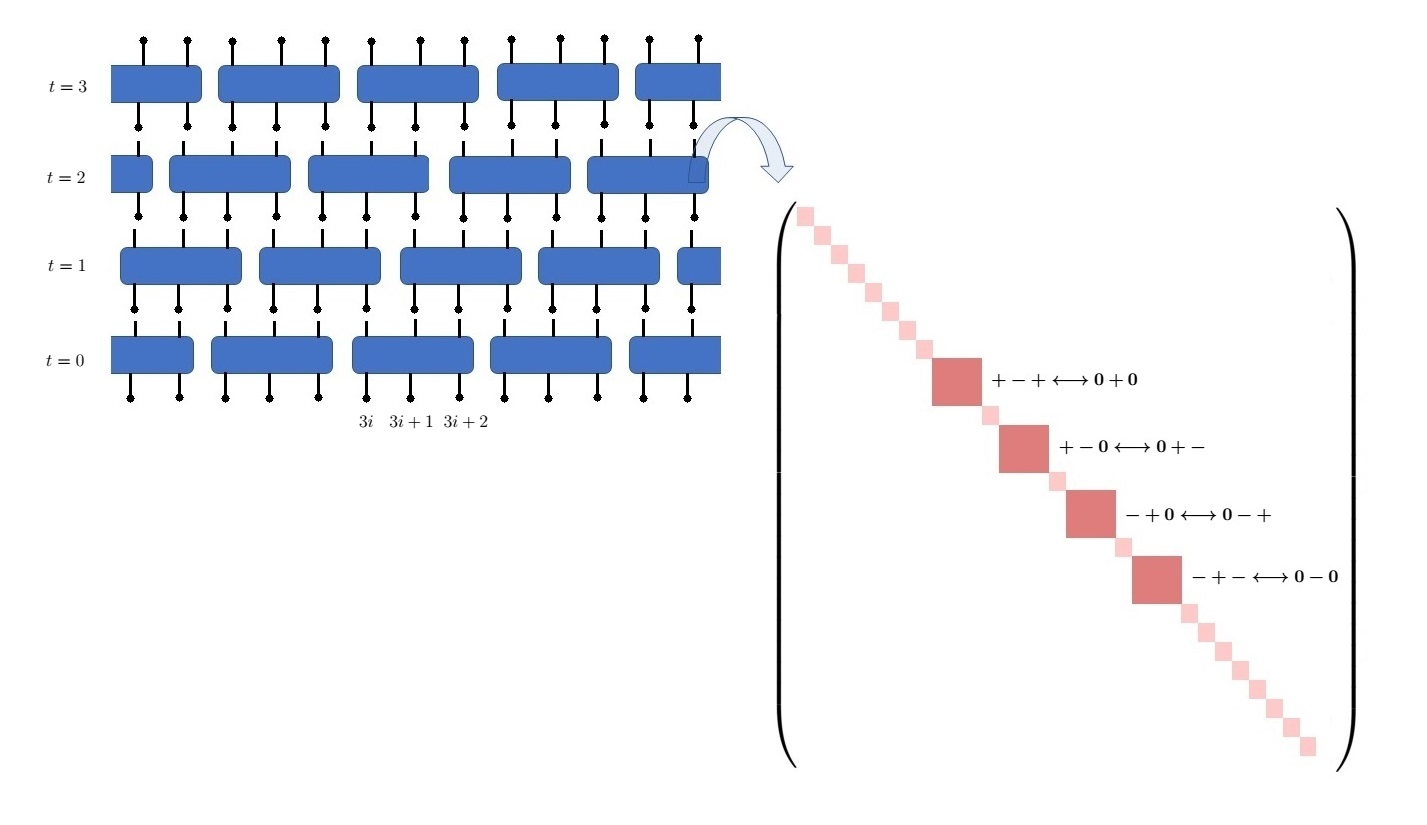
\includegraphics[width=.5\textwidth]{PaiArch}
	\caption{Architecture of the 3-site gate circuit. Each gate is a matrix of the form on the right, where each square is independently chosen from the applicable Haar distribution. The matrix is very sparse, corresponding to the small number of possible transitions. There are 4, as in Tab.~\ref{tab:pai} after adding the negative charge states. Figure from~\cite{PaiFracton}.}
	\label{fig:PaiArch}
\end{figure}
This architecture results in asymmetric lightcone velocities, but we will only look at spreading in one direction, so that will not be an issue.

\subsection{Numerical simulation} \label{sub:numeric}

As in the rest of this essay, we will discuss numerical results that are taken from another paper, unsurprisingly~\cite{PaiFracton}. We will individually show that the predictions listed in Sec.~\ref{sub:analytic} are met.

The zeroth prediction was that of fracton localization. That can be shown by starting with an initially local fracton operator and calculating its evolution. The chosen operator is $IZIII\dots$, where the only non-identity operator is on site 2. Recall that these are spin-1 systems, so 
\begin{align}
Z = \begin{pmatrix} 1 & 0 & 0 \\ 0 & 0 & 0 \\ 0 & 0 & -1 \end{pmatrix}.
\end{align}
The right-weight for this operator is shown in Fig.~\ref{fig:PaiChargeOp}.
\begin{figure}
	\centering
	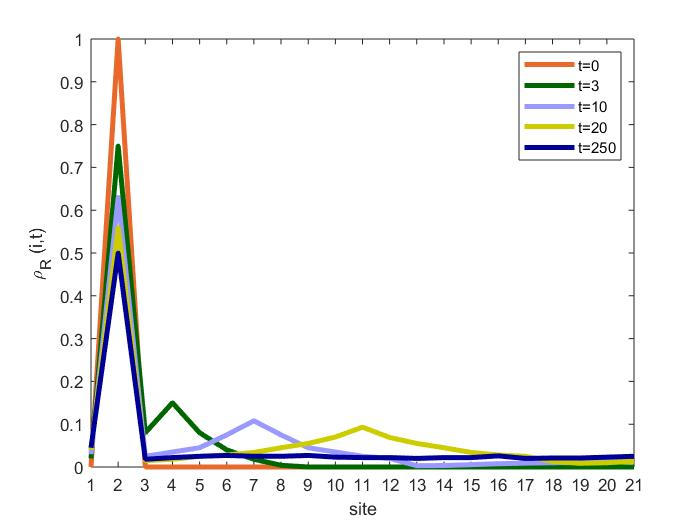
\includegraphics[width=.49\textwidth]{PaiChargeOp}
	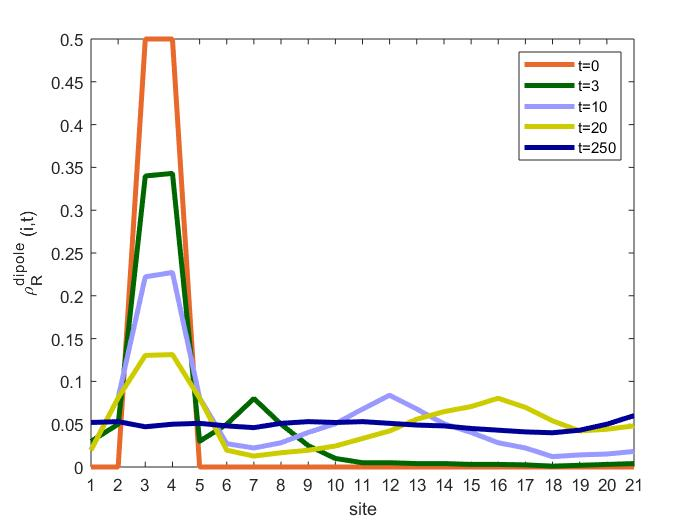
\includegraphics[width=.49\textwidth]{PaiDipoleOp}
	\caption{Operator spreading of the fracton operator and dipole operator, in a 21-site system with open boundary conditions. For the fracton, note the persistent peak at site 2, along with the propagating front. The dipole charge also has a propagating front, but the peak is nonexistent at late time. Figures from~\cite{PaiFracton}}
	\label{fig:PaiChargeOp}
\end{figure}
Note that although the peak falls to around .5, it does not fall below that value, even at late time. \note{Is this value significant?}

This is in contrast to the evolution of an initially local dipole operator. Such an operator should be the sum of adjacent fracton operators, so that its eigenstates have positive charge at one state and negative charge at the next. The chosen operator in this case is 
\begin{align}
\th{2}\left(IZIII\dots \vphantom{j}-IIZII\dots\right)
\end{align}
\note{Shouldn't it be $\th{\sqrt{2}}$?} The initial $\th{2}$ ensures that $\sum_i\rho_R(i)=1$. The time evolution of this operator is also shown in Fig.~\ref{fig:PaiChargeOp}. Note that at late time $\sum_i\rho_R(i, t)$ is essentially flat. This shows that the dipole operator is not localized, and suggests further that the late-time behavior of the fracton operator is true localization. 

To verify the first prediction, we need to move away from our familiar territory of operator spreading. The prediction is that charge density should be proportional to $\exp(R^2/2\sqrt{\pi}DCT)$. Recall that positive charge is represented by the $+1$ eigenstate of $Z$. Therefore the state with an initially local fracton is one where $\ex{Z_i}=0$ for all $i$, except for one site $j$ where $\ex{Z_j}=1$. We will once again choose $j=2$. Then we just have to show that $\ex{Z_i}\sim\exp(R^2/2\sqrt{\pi}DCT)$, $|i-j|=R$, where $\ex{Z_i}$ is evaluated with respect to a time-evolved state.

In Fig.~\ref{fig:PaiSz} we show a plot of charge density at large $t$. 
\begin{figure}
	\centering
	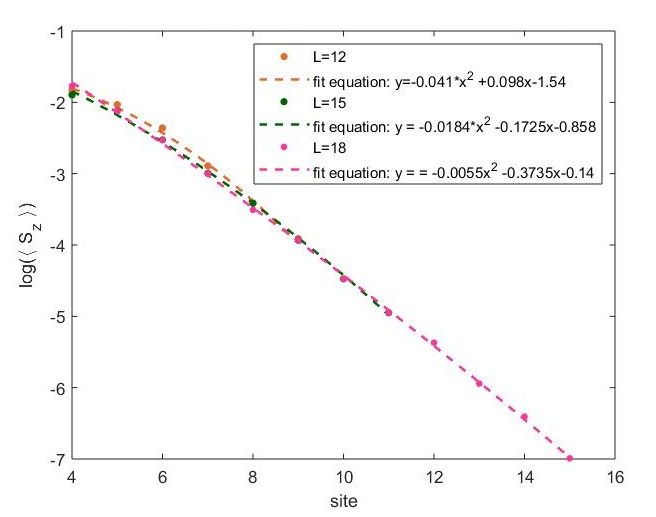
\includegraphics[width=.46\textwidth]{PaiSz}
	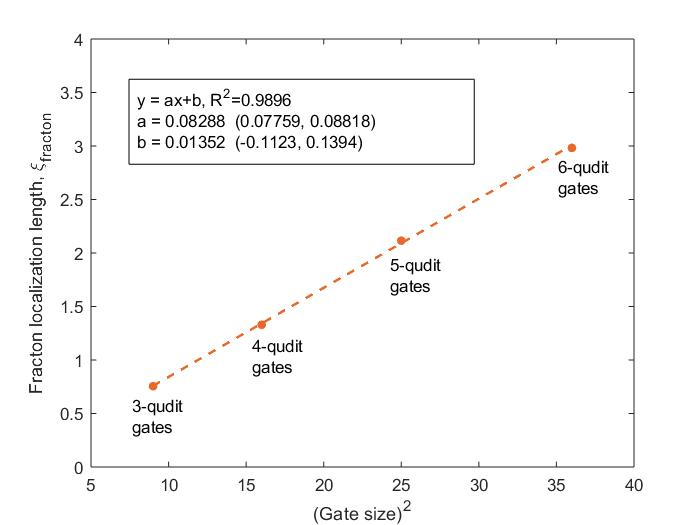
\includegraphics[width=.49\textwidth]{PaiLocLen}
	\caption{Left: Charge density at late times. If $\ex{Z_i}\sim\exp(-x^2)$, then this curve should be quadratic. It cannot be distinguished from a linear function, but the quadratic dependence is not ruled out. Right: Dependence of $\xi_\text{fracton}$ on gate size. This plot more strongly confirms the second prediction of Sec.~\ref{sub:analytic}.}
	\label{fig:PaiSz}
\end{figure}
The exponential dependence means that we can not distinguish between $\exp(-x^2)$ and $\exp(-x)$, so we count the first prediction as a maybe. 

The second prediction also depends on the spreading of charge in a single fracton state. Here, however, we have to be able to change the diffusion constant $D$ and random force $T$. We don't have many parameters left to vary in our system (the circuit is minimally structured) except for gate size. Ref.~\cite{PaiFracton} shows that both $D$ and $T$ scale as $(\text{gate size})^2$, so the second prediction reduces to
\begin{align}
\xi_\text{fracton}\sim\sqrt{DT}\sim(\text{gate size})^2.
\end{align}
$\xi_\text{fracton}$ can be extracted from the late-time charge density, as the half width at half maximum of the charge density peak.
Fig.~\ref{fig:PaiSz} also shows this relationship, confirming this prediction.

To test the last prediction, we head back to the operator spreading picture and focus on the fronts of the spreading operators. 

\begin{figure}
	\centering
	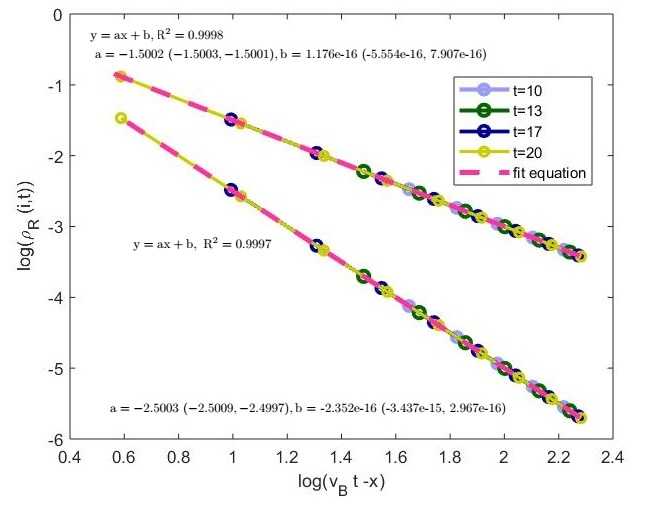
\includegraphics[width=.5\textwidth]{PaiTails}
	\caption{Behavior of the operator right weight behind the front. For the dipole operator, $\rho_R$ decreases with exponent $-3/2$ as in Sec.~\ref{sec:cons}. For the fracton operator the exponent is $-5/2$ instead. }
	\label{fig:PaiTails}
\end{figure}


\section{Results and Conclusions} \label{sec:conc}

%%%%%%%%%%%%%%%%%%%%%%%%%%%%%%%%%%%%%%%%%%%%%%%%%%%%%%%%%%%%%%%%%%
%\printbibliography
%%%%%%%%%%%%%%%%%%%%%%%%%%%%%%%%%%%%%%%%%%%%%%%%%%%%%%%%%%%%%%%%%%
\nocite{apsrev41Control}
\bibliography{../global,revtex-custom}
%%%%%%%%%%%%%%%%%%%%%%%%%%%%%%%%%%%%%%%%%%%%%%%%%%%%%%%%%%%%%%%%%%

\end{document}
